\section{Sample Web Application Implementation}\label{implementation}
I developed a web application harnessing the u2f-ref-code library ``u2f-api.js''\footnote{\href{https://github.com/google/u2f-ref-code/blob/master/u2f-gae-demo/war/js/u2f-api.js}{u2f-api.js}} library developed by Google \cite{lang2016security}. I took advantage of the tutorial of The Polyglot Developer\footnote{\url{https://www.youtube.com/watch?v=9d-mp6_vVUM}} on YouTube, and I used the Express framework for the backend, mentioned in Sec.~\ref{introduction}. I used VueJS for the frontend, harnessing the Caddy framework. I used an old version of Caddy, it does not work if you download the latest. I detailed how to download the necessary and how to setup the sample application on GitHub\footnote{\url{https://github.com/davide-giacomini/u2f-login_yubikey_express}}.

Just as a reminder, this is a sample application. It is not thought to scale for bigger purposes, but it is thought to show how to harness existing libraries to relatively easily develop a security key authentication. Therefore, it does not have a database but it simply stores the user information on a variable that gets overwritten at each registration.

The U2F protocol requires to work on \texttt{https} web pages, hence I also generated a self-generated certificate to work in localhost.

\subsection{Server Side}\label{server}
On the server side, I support four requests: a \textsc{GET} and a \textsc{POST} request for the registration and a \textsc{GET} and a \textsc{POST} request again for the authentication.

I used a library provided by the NodeJS environment called U2F to harness its functions \texttt{request}, \texttt{checkRegistration} and \texttt{checkSignature}. On GitHub there are the details on how to download each library I used.

\subsubsection{Server Registration}\label{server-registration}
See Fig.~\ref{fig:server-registration} for more details. When the user asks for registering a new security key, they perform a \textsc{GET} request to the server. The server will, in turn, use the \texttt{request} function to provide to the client an object with 1. the challenge, 2. the web origin (which is called appId in my application) and 3. the version of the U2F protocol (which in my case is the version 2).

\begin{figure}[h]
    \centering
    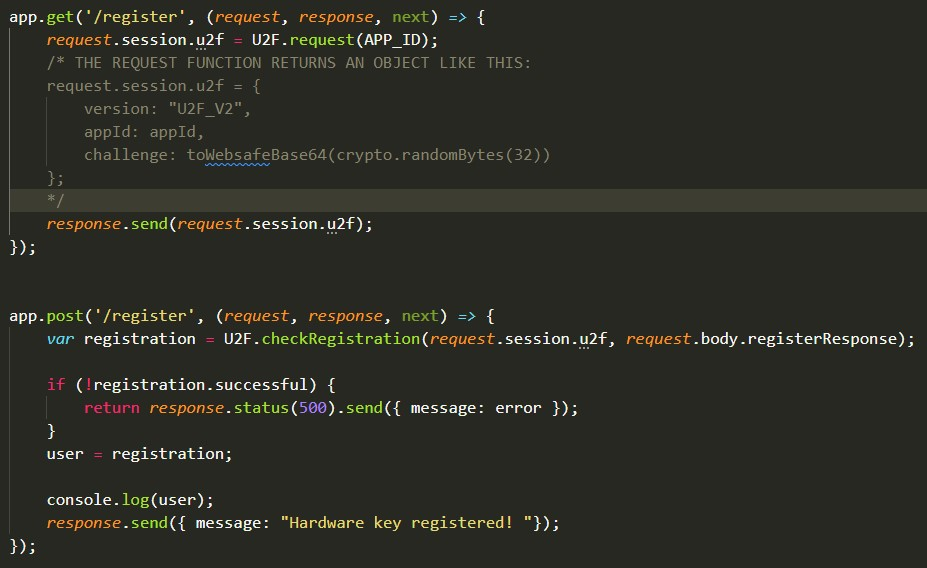
\includegraphics[width=\linewidth]{resources/register-code-server-2.jpg}
      \caption{Server registration code}
      \label{fig:server-registration}
\end{figure}

The Client will forward the information provided by the server to the device, which will generate a key pair and get back to the Client with the information listed in Sec. \ref{registration-protocol}. The security key produces a Registration Message, explained in Sec. \ref{client-registration}, which will be forwarded by the Client to the server. The server will compare the Registration Message (\texttt{registerResponse} in my application) to the object previously sent to the Client to check the presence of man-in-the-middle attacks, as explained in Sec. \ref{registration-protocol}, and, if nothing is wrong, will register the new user in its database.

\subsubsection{Server Authentication}\label{server-authentication}
Refer to Fig.~\ref{fig:server-authentication} for details. The process is very similar to the registration. Now, the server will send the key Handle previously stored along with the other information sent mentioned in Sec. \ref{server-registration}.

\begin{figure}[h]
    \centering
    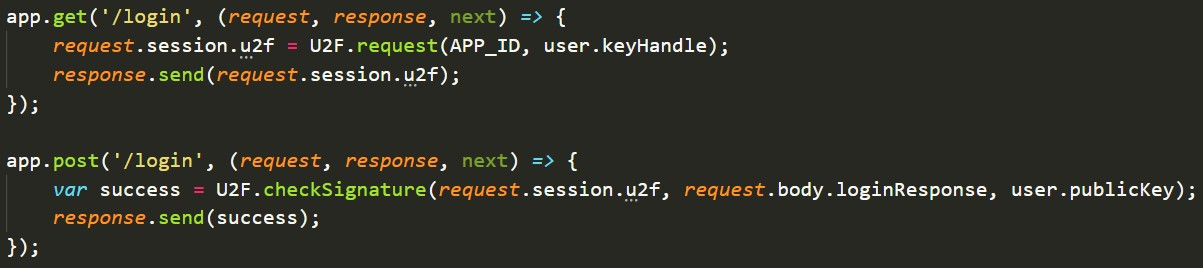
\includegraphics[width=\linewidth]{resources/login-server-code.jpg}
      \caption{Server authentication code}
      \label{fig:server-authentication}
\end{figure}

In turn, the Cient will ask the device to check everything and extract the privat key, as explained in Sec.~\ref{authentication-protocol}. The device will return an Authentication Message, detailed in Sec.~\ref{client-authentication}, to the Client, which will forward it to the server.

Finally, the server will check the signature using the public key of the user previously stored and will compare the object previously sent with the Authentication Message (Called \texttt{loginResponse} in my application).

\subsection{Client Side}
The Client side of the code harnesses the Google aforementioned API, which I manually imported in the sample application.

The API provides the method \texttt{register} and \texttt{sign}, which are used by the Client to tell the device what to do \cite{lang2016security}.

\subsubsection{Client Registration}\label{client-registration}
Refer to the code at Fig.~\ref{fig:client-registration} below. During the registration phase, the Client will get from the server the information listed in Sec.~\ref{server-registration} and will forward this information to the device. The \texttt{register} function takes as inputs the web origin (which is the object \texttt{result.data.appId} in my application), and the entire object passed along by the server (\texttt{result.data}).

\begin{figure}[h]
    \centering
    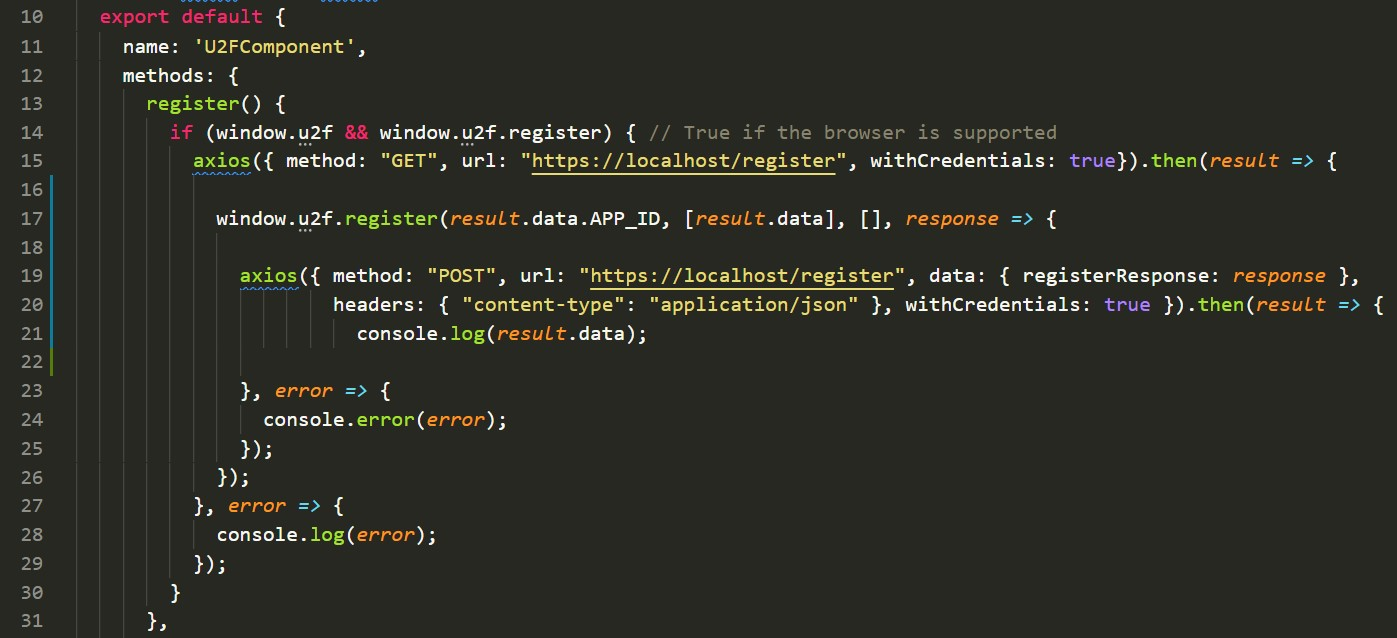
\includegraphics[width=\linewidth]{resources/register-client-code.jpg}
      \caption{Client registration code}
      \label{fig:client-registration}
\end{figure}

The device will the return the Registration Message mentioned earlier. This message contains the user public key, the key Handle, the attestation certificate and the signature over some information (Fig.~\ref{fig:registration-message}). The Registration Message will then be forwarded by the Client to the server, which will use it under the name \texttt{registerResponse}, as seen in Sec.~\ref{server-registration}.

\begin{figure}[h]
    \centering
    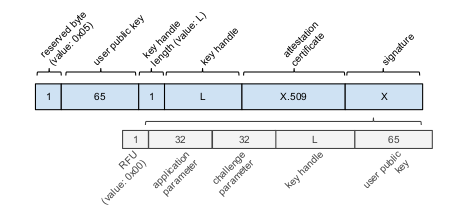
\includegraphics[width=\linewidth]{resources/registration-message.png}
      \caption{Registration Message}
      \label{fig:registration-message}
\end{figure}

\subsubsection{Client Authentication}\label{client-authentication}
Refer to Fig.~\ref{fig:client-authentication}. The pattern is identical to the registration phase. Here, the function \texttt{sign} takes as inputs the web origin (\texttt{result.data.appId}), the challenge (\texttt{result.data.challenge}), and the entire object sent by the server (\texttt{result.data}).

\begin{figure}[h]
    \centering
    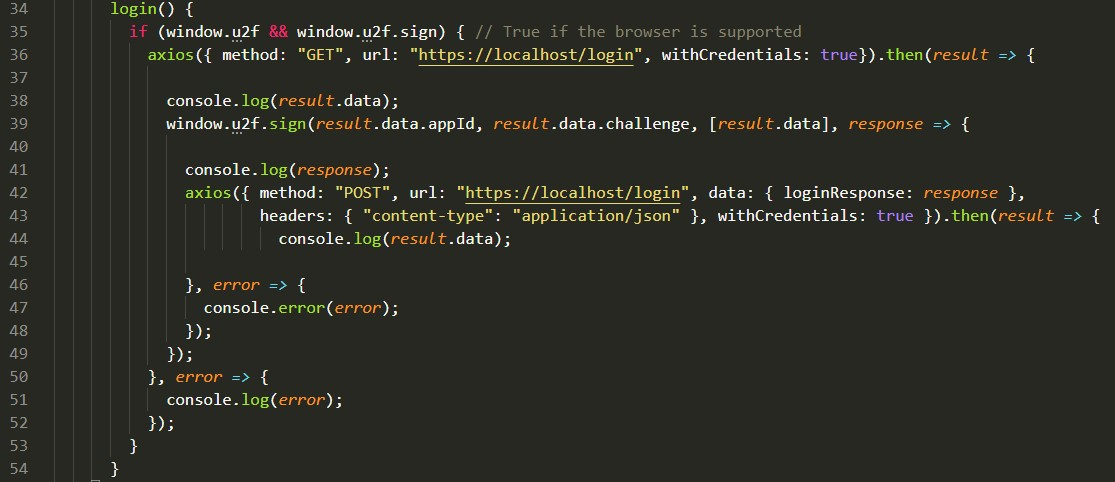
\includegraphics[width=\linewidth]{resources/login-client-code.jpg}
      \caption{Client authentication code}
      \label{fig:client-authentication}
\end{figure}

The security key then returns the Authentication Message mentioned earlier (Fig.~\ref{fig:authentication-message}), which contains the counter and the signature over some parameters, among them the Test of User Presence.

\begin{figure}[h]
    \centering
    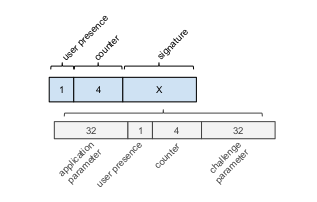
\includegraphics[width=0.5\linewidth]{resources/authentication-message.png}
    \caption{Authentication Message}
    \label{fig:authentication-message}
\end{figure}